\documentclass[12pt]{article}

% French
\usepackage[utf8]{inputenc}
\usepackage[T1]{fontenc}
\usepackage[french]{babel}

\usepackage{hyperref}
\usepackage{pdfpages}
\usepackage{float}
\usepackage{geometry}
\usepackage{tikz}
\usepackage{eurosym}

\usepackage{multirow}
\usepackage{datetime}

\usepackage{titlesec}

\titleformat*{\section}{\LARGE\bfseries}
\titleformat*{\subsection}{\Large\bfseries}
\titleformat*{\subsubsection}{\large\bfseries}
\titleformat*{\paragraph}{\large\bfseries}
\titleformat*{\subparagraph}{\large\bfseries}


\geometry{margin=2.5cm}

\definecolor{darkgreen}{RGB}{0,130,0}
\definecolor{darkblue}{RGB}{0,0,130}

\newcommand{\gameName}{\textit{Lands of Azerith}}
\newcommand{\companyName}{Stonks Industries}
% \newcommand{\progressbar}[1]{
%     \begin{tikzpicture}
%         \fill[black!30] (0,0) rectangle (#1/100*2cm, 0.2);
%         \draw (0,0) rectangle (2cm, 0.2);
%     \end{tikzpicture}
%     \small{#1\%}
% }

\title{
    Rapport de la seconde soutenance \\
    \textbf{\gameName} \\
    \vspace{0.5cm}
    
\includegraphics[width=5cm]{0.format/logo.png}
    \vspace{4.2cm}
}
\author{
    Ayemane Bouarbi \\
    \texttt{ayemane.bouarbi@epita.fr}
    \vspace{0.5cm}\and
    Louise Fussien \\
    \texttt{louise.fussien@epita.fr}
    \vspace{0.5cm}\and
    Michaël Museux \\
    \texttt{michael.museux@epita.fr}
    \vspace{0.5cm}\and
    Martin Pasquier \\
    \texttt{martin.pasquier@epita.fr}
}

\date{
    \vspace{1.5cm}
    \textbf{\companyName} \\
    \vspace{0.3cm}
    \textbf{EPITA} \\
    \vspace{1.5cm}
    \today
}

\begin{document}

\begin{titlepage}
    \maketitle
    \thispagestyle{empty} % Remove page number from title page
\end{titlepage}

\newpage
\thispagestyle{empty}
\mbox{}

\newpage
\tableofcontents

\newpage
\section{Introduction}
% Dans le cadre de notre formation à EPITA, nous avons entrepris un projet ambitieux visant à développer un jeu vidéol. Ce projet, qui s'étend sur l'ensemble de l'année académique, nous a permis d'acquérir et de perfectionner nos compétences en programmation, en design de jeux et en gestion de projet. La soutenance de fin d'année marque l'aboutissement de nos efforts collectifs et individuels. Elle offre une occasion privilégiée de présenter l'évolution du projet, les défis surmontés et les résultats obtenus.



\newpage
\section{Le projet}

\subsection{Changements depuis la dernière soutenance}
% \input{1.project/changes.tex}

\subsection{Site web}
% \input{1.project/website.tex}

\subsection{Cahier des Charges Technique}
% % This file CAN NOT be compiled on its own
% It is included by ../Book_of_Specifications.tex

% TODO Update the technical book

Les deux prochaines pages sont dédiées au cahier des charges technique.
Ce document détaille les contraintes et les caractéristiques techniques nécessaires pour répondre aux besoins du projet.
Il synthétise toutes les réponses aux questions techniques que l'on peut se poser sur le projet.
\\

Le cahier des charges technique est divisé en deux parties.
La première partie détaille les spécificités du jeu et les choix techniques qui ont été réalisés. 
La deuxième partie donne des informations sur la repartition des tâches et leur avancement.
\\

Des changements ont été apportés au cahier des charges technique depuis sa dernière version.
Le nom du jeu a été modifié, le départ de Mohamed Aziz et Alexandre a été pris en compte, et des changements ont été apportés au diagramme de Gantt pour refléter l'avancé du projet.
\\

Le dernier cahier des charges technique, intégré dans ce rapport final, reflète ces ajustements. Il décrit non seulement 
les spécifications finales du jeu telles qu'elles ont évolué tout au long du processus, mais aussi les décisions stratégiques prises pour surmonter les défis rencontrés.



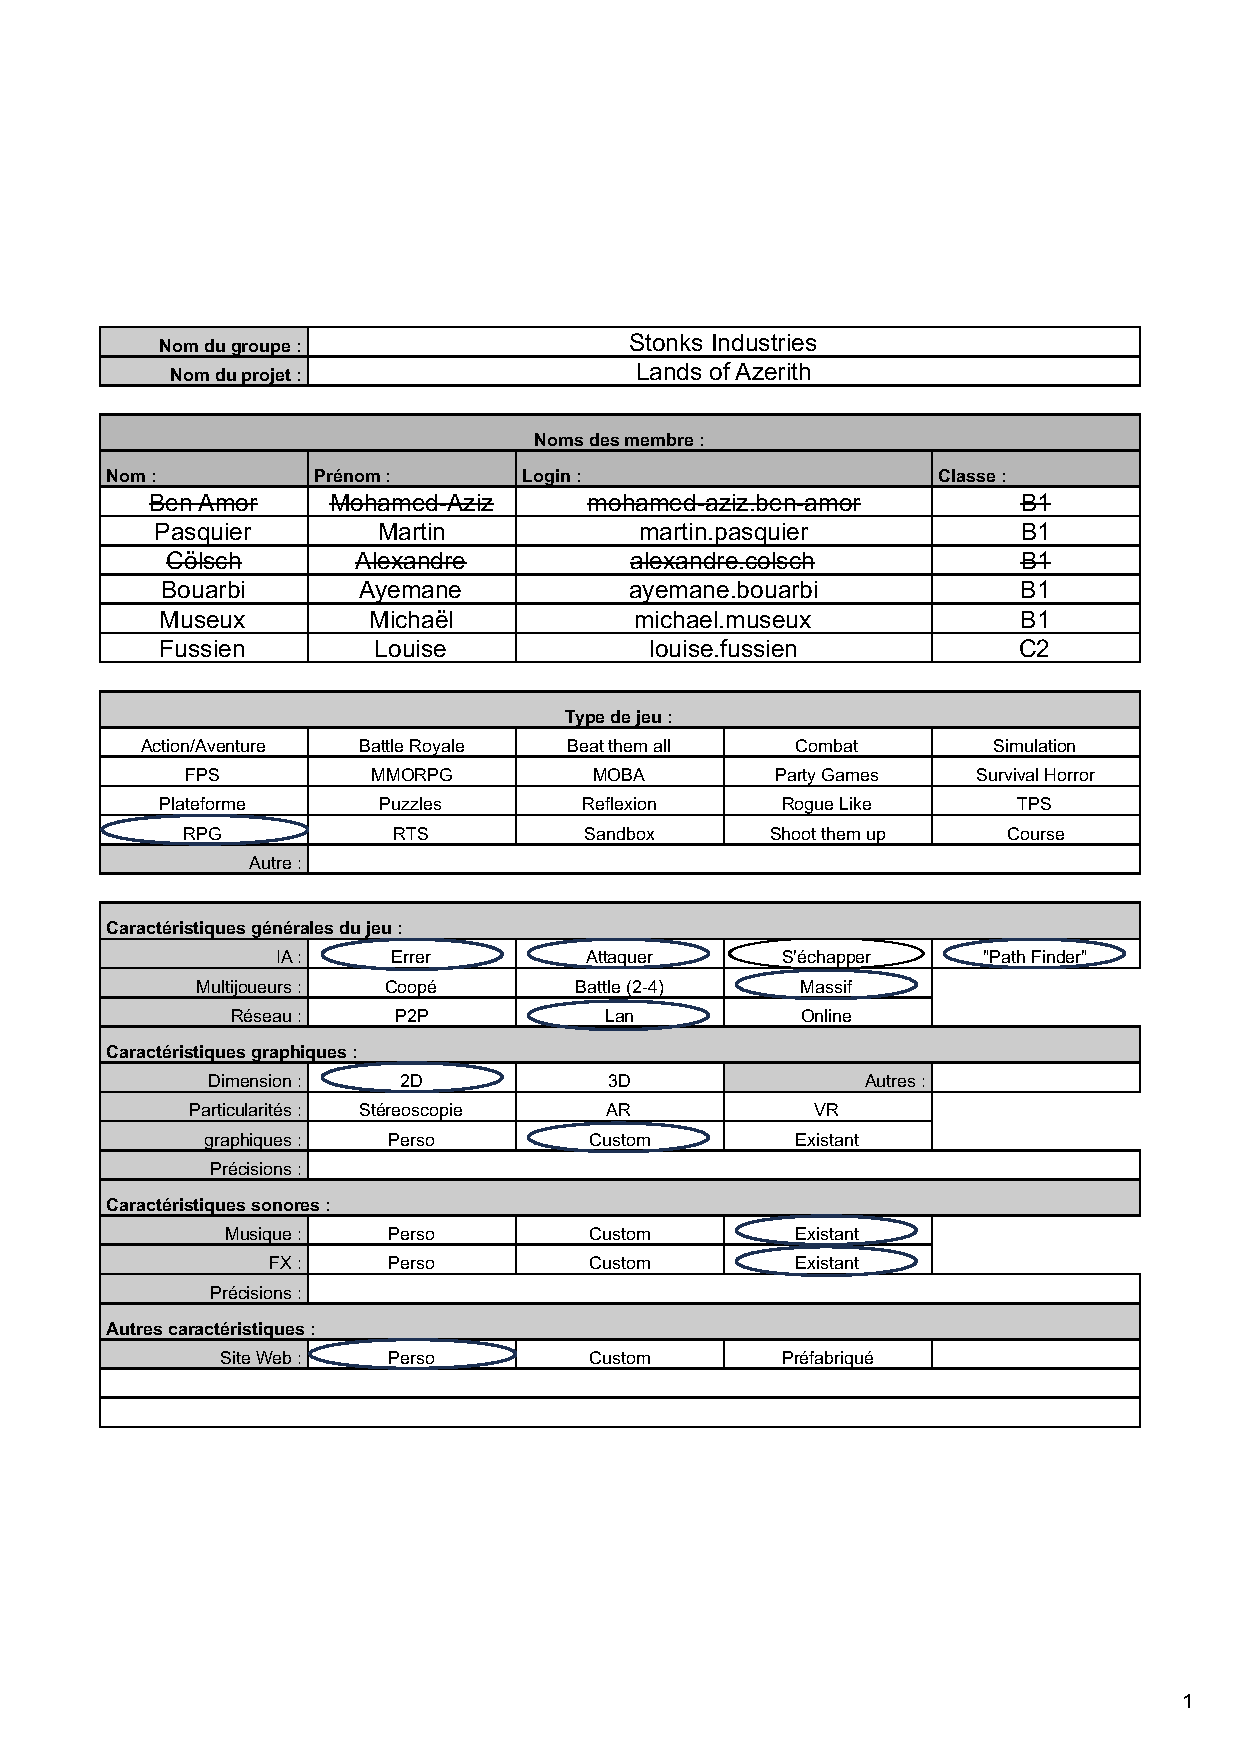
\includepdf[pages=1]{technical_book/page-1.pdf}

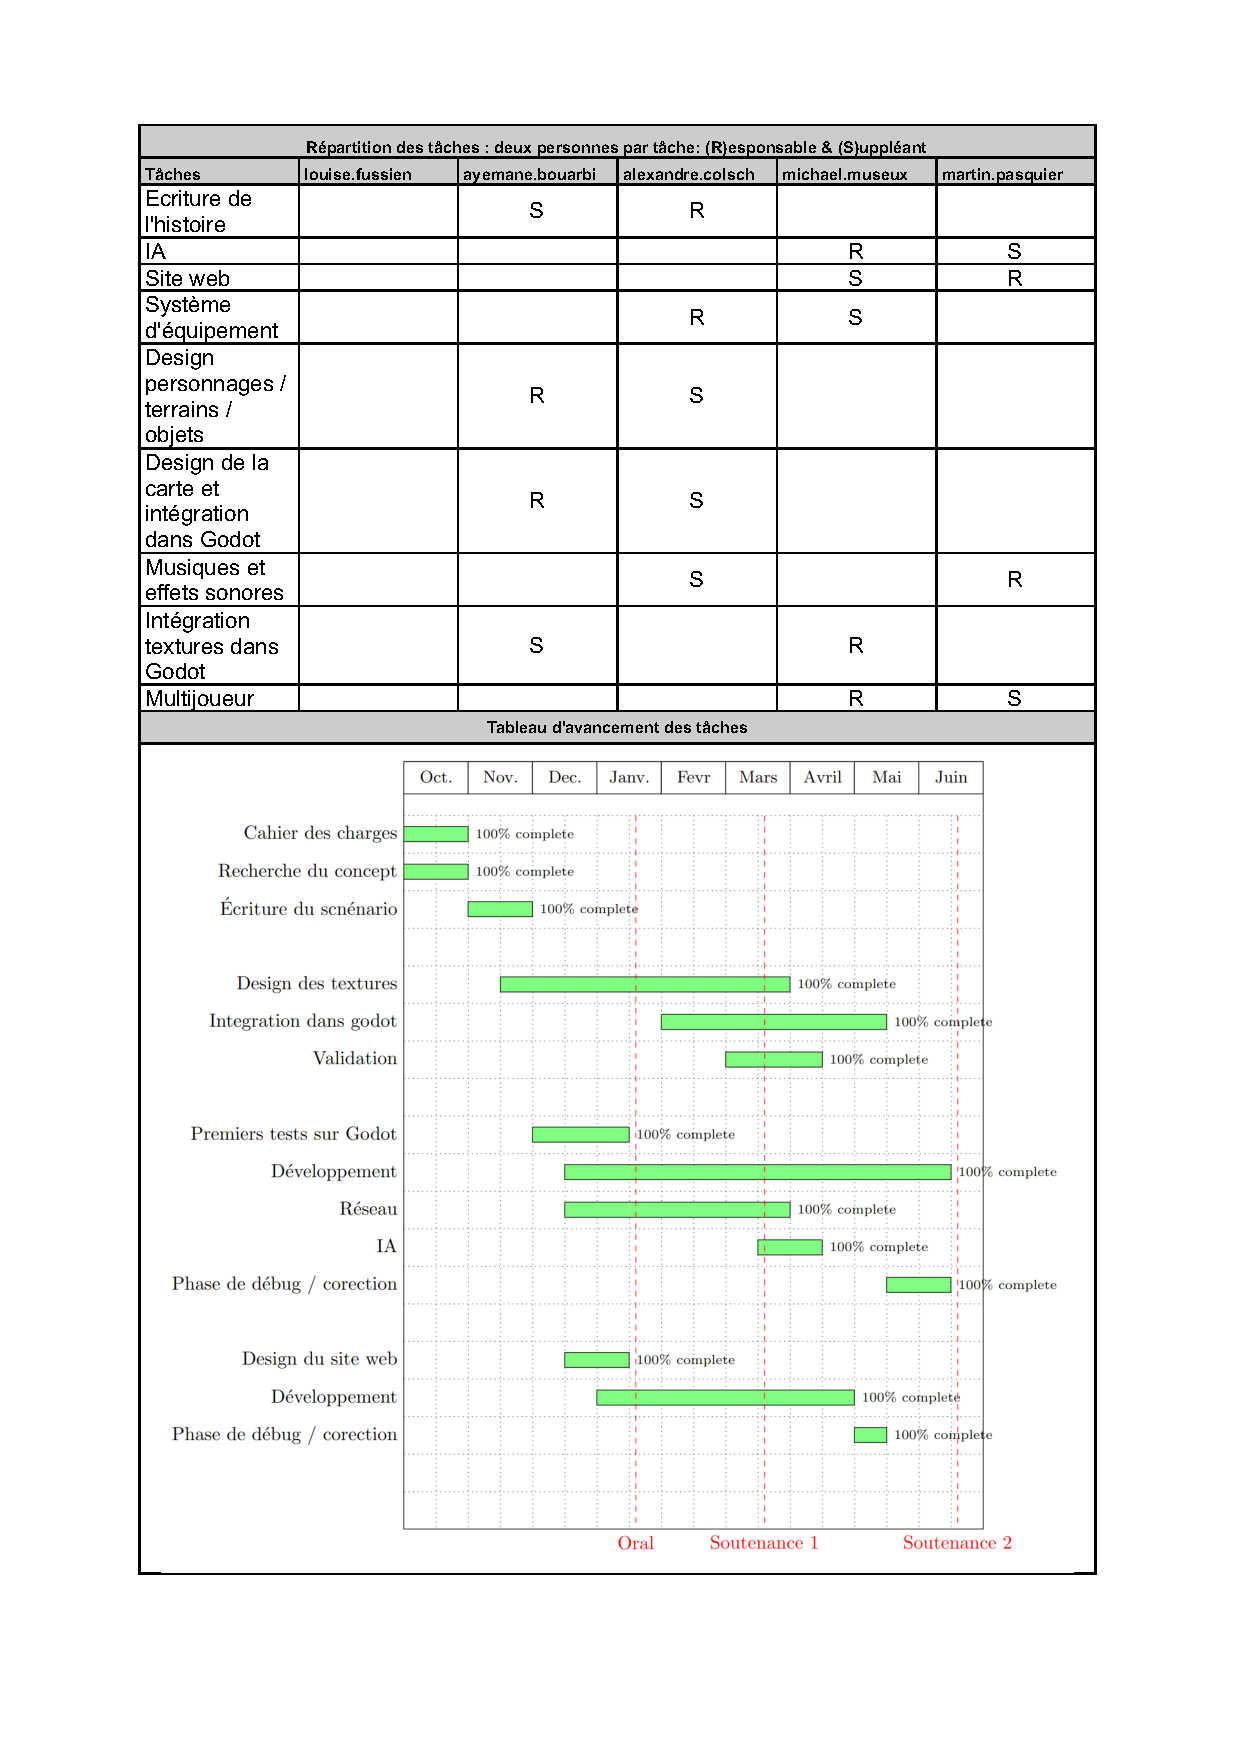
\includepdf[pages=1]{technical_book/page-2.pdf}



\newpage
\section{Le jeu}

\subsection{IA, Mécaniques de gameplay}
% \input{2.game/gameplay.tex}

\subsection{Design}
% \input{2.game/design.tex}

\subsection{Histoire}
% \input{2.game/story.tex}

\subsection{Son et musique}
% \input{2.game/sound.tex}


\newpage
\section{Conclusion}
% \input{0.format/conclusion.tex}

% Logo of the company
\centering
\vspace*{1.8cm}

\includegraphics[width=3cm]{0.format/logo.png}

% Day and time of the last update
\vspace*{1cm}
Last updated on \today{} at \currenttime.

\end{document}
